\documentclass[11pt,a4paper]{article}

\usepackage[utf8]{inputenc}
\usepackage[margin=1in]{geometry}
\usepackage{amsmath,amssymb,amsthm}
\usepackage{graphicx}
\usepackage{booktabs}
\usepackage{xcolor}
\usepackage{hyperref}
\usepackage{microtype}
\usepackage{cite}
\usepackage{bm}
\usepackage{caption}
\usepackage{subcaption}

% Hyperref setup
\hypersetup{
    colorlinks=true,
    linkcolor=blue!70!black,
    citecolor=blue!70!black,
    urlcolor=blue!70!black
}

% Theorem environments
\theoremstyle{plain}
\newtheorem{theorem}{Theorem}[section]
\newtheorem{lemma}[theorem]{Lemma}
\newtheorem{proposition}[theorem]{Proposition}
\newtheorem{corollary}[theorem]{Corollary}

\theoremstyle{definition}
\newtheorem{definition}[theorem]{Definition}
\newtheorem{remark}[theorem]{Remark}
\newtheorem{example}[theorem]{Example}

\title{\textbf{Exact Rational Perturbation Theory, Monotonicity Phase Transitions, and Fast All-Pairs Optimization for Kemeny's Constant in Complex Networks}}

\author{
    \textbf{Rajveersinh Vishal Pardeshi}\\[0.5em]
    \textit{Independent Researcher}
}

\date{\today}

\begin{document}

\maketitle

\begin{abstract}
Kemeny's constant is a fundamental spectral invariant measuring the expected transit time between random states in a Markov chain. In complex networks, adding an edge can paradoxically increase Kemeny's constant---an analogue of Braess's paradox for random walks. Prior investigations have either been confined to special graph families (such as trees or complete multipartite graphs) under unit edge additions or relied on infinitesimal directional derivatives. In this paper, we establish the exact algebraic closed-form perturbation theory of Kemeny's constant under finite rank-one edge modifications for arbitrary finite, connected, undirected weighted graphs. We prove that the change in Kemeny's constant $\Delta K(G; u, v, w)$ under an added edge $(u, v)$ with continuous weight $w > 0$ is strictly a rational function of the form $\frac{w(A_0 + A_1 w)}{2m(m+w)(1+w\Omega(u, v))}$, where $\Omega(u, v)$ is the effective resistance. Remarkably, we prove an exact algebraic cancellation theorem demonstrating that the quadratic numerator coefficient $A_2$ vanishes identically ($A_2 \equiv 0$) across all graphs and vertex pairs due to an underlying $2 \times 2$ determinantal identity of the Laplacian Moore-Penrose pseudoinverse. This linearity of the numerator gives rise to four mutually exclusive topological regimes, including the discovery of a \textit{Weight-Induced Braess Phase Transition}: non-edges that are strictly favorable for small capacities ($w < w^*$) but become Braess bottlenecks for large capacities ($w > w^*$), with an exact closed-form threshold $w^*(u, v) = -A_0 / A_1$. Furthermore, by introducing the symmetric metric matrix $M = L^\dagger D L^\dagger$, we design an exact all-pairs deterministic algorithm that computes $\Delta K(u, v, w)$ for all $\binom{n}{2}$ candidate pairs in $\mathcal{O}(n^3)$ precomputation plus $\mathcal{O}(1)$ query time per pair, achieving an $n^2$ computational acceleration over brute-force recomputation. In-process benchmarks confirm empirical speedups exceeding $13,000\times$ on networks of 50 vertices, while topological audits reveal that the Weight-Induced Braess regime is prevalent, comprising up to $70.2\%$ of non-edges in trees and $28.2\%$ in modular barbell networks.
\end{abstract}

\textbf{Keywords:} Kemeny's constant, Random walks, Spectral graph theory, Braess's paradox, Effective resistance, Graph Laplacian, Perturbation theory, Network optimization.

\section{Introduction}
\label{sec:intro}

Random walks on graphs provide a cornerstone for modern network science, distributed consensus protocols, spectral partitioning, and diffusion processes on complex systems~\cite{doyle1984random,spielman2011graph}. A central structural invariant characterizing the global navigability and mixing efficiency of a finite, connected, undirected network $G = (V, E, W)$ is \textit{Kemeny's constant}, denoted by $K(G)$~\cite{kemeny1960finite}. Originally introduced by John Kemeny and Laurie Snell for finite Markov chains, $K(G)$ possesses the remarkable property of representing the expected number of steps required for a random walker, starting at \textit{any} arbitrary vertex $i \in V$, to first reach a destination node $j \in V$ sampled according to the stationary distribution $\pi$:
\begin{equation}
    K(G) = \sum_{j \in V} \pi_j H(i, j), \quad \forall i \in V,
\end{equation}
where $H(i, j)$ denotes the mean first hitting time from vertex $i$ to vertex $j$. The fact that this sum is entirely independent of the starting vertex $i$ makes Kemeny's constant an intrinsic spectral invariant of the network. Spectrally, if $1 = \lambda_1 > \lambda_2 \ge \cdots \ge \lambda_n \ge -1$ are the eigenvalues of the random walk transition probability matrix $P = D^{-1} W$, Kemeny's constant is expressed as:
\begin{equation}
    K(G) = \sum_{i=2}^n \frac{1}{1 - \lambda_i}.
\end{equation}
Lower values of $K(G)$ correspond to fast mixing, high connectivity, and absence of bottlenecks, while larger values indicate sluggish traversal and segregated modular components.

In physical and communication networks, a pervasive operational goal is capacity expansion: identifying candidate edges whose addition or reinforcement will maximally reduce transit times and enhance network throughput~\cite{ghosh2008minimizing}. In electrical resistor networks, Rayleigh's Monotonicity Law guarantees that adding a resistor or increasing edge conductance strictly decreases (or preserves) the effective resistance between every pair of nodes, ensuring that the total effective resistance (the Kirchhoff index) is strictly monotone decreasing and convex in edge weights~\cite{ghosh2008minimizing,klein1993resistance}.

In sharp contrast to electrical networks, random walks on graphs can exhibit a structural pathology known as the \textit{Braess Paradox for Random Walks}~\cite{hu2019complete,kirkland2023edge,bini2023edge}: adding a new edge $e = (u, v)$ to a connected graph $G$ can cause Kemeny's constant to strictly \textit{increase} ($K(G + e) > K(G)$). Although the added link locally decreases the pairwise resistance distance $\Omega(u, v)$, it simultaneously perturbs the stationary distribution $\pi$ and vertex degree weights, potentially trapping random walkers inside poorly connected peripheral modules and increasing global transit times. An edge whose addition increases $K(G)$ is termed a \textit{Braess edge}~\cite{hu2019complete}.

Despite significant interest, existing literature on Kemeny edge perturbations suffers from two fundamental limitations:
\begin{enumerate}
    \item \textbf{Restricted Topological Scope and Unit Weights:} Existing analytical characterizations of Braess edges have been derived almost exclusively for highly specialized graph families under unweighted additions ($w = 1$). For example, Hu and Kirkland~\cite{hu2019complete} established algebraic conditions for complete multipartite and complete split graphs, while Kirkland et al.~\cite{kirkland2023edge} recently proved asymptotic bounds specifically for adding an edge to a tree. The exact algebraic response of general graphs under continuous edge weights $w \in (0, \infty)$ has remained unformulated.
    \item \textbf{The Infinitesimal vs.\ Finite Capacity Discrepancy:} To circumvent combinatorial enumeration, recent works have focused on the infinitesimal directional derivative $\left.\frac{\partial K}{\partial w_{uv}}\right|_{w=0}$ as a measure of edge centrality~\cite{bini2023edge}. However, as we demonstrate in this paper, infinitesimal sensitivities can be deeply misleading: an edge can have a negative directional derivative (suggesting that adding capacity will improve network performance), yet for finite capacities $w > w^*$, the very same edge increases Kemeny's constant, worsening global performance.
\end{enumerate}

\subsection{Our Contributions}
In this work, we resolve these open problems through the following contributions:
\begin{enumerate}
    \item \textbf{The Exact Rational Perturbation Theorem (Theorem~\ref{thm:rational_perturbation}):} We derive the exact closed-form algebraic formula for the change in Kemeny's constant $\Delta K(G; u, v, w) = K(G + w e_{uv}) - K(G)$ for \textit{any} connected, undirected weighted graph under an arbitrary continuous perturbation $w > 0$. We prove that $\Delta K(w)$ is a rational function with quadratic denominator:
    \begin{equation}
        \Delta K(G; u, v, w) = \frac{w (A_0 + A_1 w)}{2m(m + w)(1 + w \Omega(u, v))}.
    \end{equation}
    \item \textbf{The Exact Algebraic Cancellation Theorem (Theorem~\ref{thm:cancellation}):} We discover and prove that the quadratic numerator coefficient $A_2$ vanishes identically ($A_2 \equiv 0$) for all graphs and all pairs of vertices. This cancellation arises from a fundamental algebraic identity connecting the graph volume, degree couplings, and the $2 \times 2$ principal submatrix determinant of the Moore-Penrose pseudoinverse $L^\dagger$.
    \item \textbf{The Four-Regime Classification and Weight-Induced Braess Paradox (Theorem~\ref{thm:regimes}):} Because the numerator $N(w) = A_0 + A_1 w$ is strictly linear, we partition all candidate edge modifications into four exact regimes. In particular, we discover the \textit{Weight-Induced Braess Phase Transition}: edges for which $A_0 < 0$ and $A_1 > 0$, yielding a unique critical weight $w^*(u, v) = -A_0 / A_1$. For $w < w^*$, the edge is favorable ($\Delta K < 0$); for $w > w^*$, it becomes Braess ($\Delta K > 0$), with a unique interior optimal capacity $w_{\mathrm{opt}} \in (0, w^*)$ that strictly minimizes Kemeny's constant.
    \item \textbf{Fast All-Pairs Optimization Algorithm (Theorem~\ref{thm:complexity}):} By introducing the symmetric metric matrix $M = L^\dagger D L^\dagger$, we prove that the dipole energy term $x^T D x = M_{uu} + M_{vv} - 2 M_{uv}$ can be evaluated in $\mathcal{O}(1)$ time. This yields an exact deterministic algorithm that evaluates all $\binom{n}{2}$ candidate edge modifications in $\mathcal{O}(n^3)$ precomputation plus $\mathcal{O}(1)$ query time per pair, achieving an $n^2$ speedup over the naive $\mathcal{O}(n^5)$ recomputation.
    \item \textbf{Reproducible Empirical Validation:} We perform extensive in-process execution benchmarks and topological audits across canonical graph models and real-world networks (including Zachary's Karate Club). Our empirical results establish that Weight-Induced Braess transitions dominate in sparse and modular networks, accounting for $70.2\%$ of non-edges in random trees and $28.2\%$ in barbell graphs.
\end{enumerate}

\section{Problem Formulation and Related Work}
\label{sec:formulation}

\subsection{Preliminaries and Notation}
Let $G = (V, E, W)$ be a finite, connected, undirected graph with vertex set $V = \{1, 2, \dots, n\}$ and non-negative symmetric edge weight matrix $W \in \mathbb{R}^{n \times n}_{\ge 0}$, where $W_{ij} = W_{ji} > 0$ if and only if $\{i, j\} \in E$, and $W_{ii} = 0$. The degree of vertex $i$ is $d_i = \sum_{j=1}^n W_{ij}$, and $D = \operatorname{diag}(d_1, \dots, d_n)$ denotes the diagonal degree matrix. The total volume of the graph is $2m = \sum_{i=1}^n d_i = \mathbf{1}^T d$, where $\mathbf{1} = (1, 1, \dots, 1)^T \in \mathbb{R}^n$.

The combinatorial graph Laplacian is defined as $L = D - W$. Because $G$ is undirected and connected, $L$ is a symmetric, positive semidefinite matrix with nullspace $\operatorname{Null}(L) = \operatorname{span}(\mathbf{1})$. Its eigenvalues satisfy $0 = \mu_1 < \mu_2 \le \cdots \le \mu_n$, where $\mu_2 > 0$ is the algebraic connectivity of $G$. The Moore-Penrose pseudoinverse of $L$ is denoted by $L^\dagger$. It satisfies $L L^\dagger = L^\dagger L = I - \frac{1}{n} \mathbf{1} \mathbf{1}^T = P_{\mathbf{1}^\perp}$, the orthogonal projector onto $\mathbf{1}^\perp$.

The discrete-time random walk on $G$ is governed by the transition probability matrix $P = D^{-1} W$. The stationary distribution is given by the probability vector $\pi = \frac{1}{2m} d$, which satisfies $\pi^T P = \pi^T$. The effective resistance (or resistance distance) between vertices $u$ and $v$ is given by~\cite{klein1993resistance}:
\begin{equation}
    \Omega(u, v) = (e_u - e_v)^T L^\dagger (e_u - e_v) = L^\dagger_{uu} + L^\dagger_{vv} - 2 L^\dagger_{uv},
\end{equation}
where $e_i \in \mathbb{R}^n$ is the $i$-th standard basis vector.

\subsection{Related Work}
A summary of the closest prior work and the specific advances established in this paper is detailed in Table~\ref{tab:literature}.

\begin{table}[htbp]
\centering
\small
\caption{Comparison of our contributions with key prior literature on Kemeny edge variations.}
\label{tab:literature}
\begin{tabular}{@{}p{3.2cm}p{3.8cm}p{3.5cm}p{4.2cm}@{}}
\toprule
\textbf{Reference} & \textbf{Graph Scope} & \textbf{Perturbation Type} & \textbf{Primary Result vs.\ Our Advance} \\
\midrule
Hu \& Kirkland (2019)~\cite{hu2019complete} & Complete multipartite \& split graphs & Discrete unit addition ($w=1$) & Classified Braess non-edges via characteristic polynomials. \textit{Advance: We generalize to arbitrary connected graphs for all continuous $w > 0$.} \\
\addlinespace
Kirkland et al. (2024)~\cite{kirkland2023edge} & Trees ($T_n$) & Discrete unit addition ($w=1$) & Proved extremal bounds on trees ($\Delta K \in [-\frac{3}{16}n^2, \frac{2}{3}n]$). \textit{Advance: We provide the exact closed-form rational function for any topology.} \\
\addlinespace
Bini et al. (2023)~\cite{bini2023edge} & General connected graphs & Infinitesimal derivative ($w \to 0$) & Formulated $\left.\frac{\partial K}{\partial w}\right|_{w=0}$ for edge centrality. \textit{Advance: We resolve finite-capacity Braess transitions where the derivative fails.} \\
\addlinespace
Ghosh et al. (2008)~\cite{ghosh2008minimizing} & General connected graphs & Convex allocation of weights & Proved total effective resistance is convex and strictly monotone. \textit{Advance: We characterize the exact non-monotone phase space of Kemeny's constant.} \\
\bottomrule
\end{tabular}
\end{table}

\section{Foundations of Kemeny's Constant}
\label{sec:foundations}

We begin by establishing a closed-form matrix representation of Kemeny's constant in terms of the Moore-Penrose pseudoinverse $L^\dagger$.

\begin{lemma}[Laplacian Representation of Kemeny's Constant]
\label{lem:kemeny_laplacian}
Let $G = (V, E, W)$ be a connected, undirected graph with degree vector $d$, diagonal degree matrix $D$, total volume $2m = \mathbf{1}^T d$, and Laplacian pseudoinverse $L^\dagger$. Then:
\begin{equation}
    K(G) = \operatorname{Tr}(D L^\dagger) - \frac{1}{2m} d^T L^\dagger d.
\end{equation}
\end{lemma}

\begin{proof}
By the electrical resistance formulation of hitting times in finite Markov chains~\cite{doyle1984random,hunter2014role}, Kemeny's constant can be expressed as a weighted sum over all pairwise effective resistances:
\begin{equation}
    K(G) = \frac{1}{4m} \sum_{p=1}^n \sum_{q=1}^n d_p d_q \Omega(p, q).
\end{equation}
Expanding the effective resistance $\Omega(p, q) = L^\dagger_{pp} + L^\dagger_{qq} - 2 L^\dagger_{pq}$:
\begin{align}
    \sum_{p=1}^n \sum_{q=1}^n d_p d_q \Omega(p, q) &= \sum_{p=1}^n \sum_{q=1}^n d_p d_q (L^\dagger_{pp} + L^\dagger_{qq} - 2 L^\dagger_{pq}) \nonumber \\
    &= \left(\sum_{q=1}^n d_q\right) \sum_{p=1}^n d_p L^\dagger_{pp} + \left(\sum_{p=1}^n d_p\right) \sum_{q=1}^n d_q L^\dagger_{qq} - 2 \sum_{p=1}^n \sum_{q=1}^n d_p d_q L^\dagger_{pq}.
\end{align}
Since $\sum_{p=1}^n d_p = 2m$ and $\sum_{p=1}^n d_p L^\dagger_{pp} = \operatorname{Tr}(D L^\dagger)$, we obtain:
\begin{equation}
    \sum_{p=1}^n \sum_{q=1}^n d_p d_q \Omega(p, q) = 2m \operatorname{Tr}(D L^\dagger) + 2m \operatorname{Tr}(D L^\dagger) - 2 d^T L^\dagger d = 4m \operatorname{Tr}(D L^\dagger) - 2 d^T L^\dagger d.
\end{equation}
Dividing by $4m$ yields:
\begin{equation}
    K(G) = \frac{4m \operatorname{Tr}(D L^\dagger) - 2 d^T L^\dagger d}{4m} = \operatorname{Tr}(D L^\dagger) - \frac{1}{2m} d^T L^\dagger d,
\end{equation}
completing the proof.
\end{proof}

\section{Main Results: Exact Rational Perturbation Theory}
\label{sec:main_results}

We now consider perturbing the graph $G$ by adding an edge between non-adjacent vertices $u$ and $v$ (or reinforcing an existing edge) with weight $w > 0$. The perturbed adjacency matrix is $W_{\mathrm{new}} = W + w (e_u e_v^T + e_v e_u^T)$, the degree vector becomes $d_{\mathrm{new}} = d + w(e_u + e_v)$, and the perturbed Laplacian is:
\begin{equation}
    L_{\mathrm{new}} = L + w (e_u - e_v)(e_u - e_v)^T = L + w b b^T,
\end{equation}
where $b = e_u - e_v \in \mathbb{R}^n$.

\begin{lemma}[Rank-One Pseudoinverse Update on $\mathbf{1}^\perp$]
\label{lem:sherman_morrison_pinv}
Let $b = e_u - e_v$. For any $w > 0$, the Moore-Penrose pseudoinverse of $L_{\mathrm{new}} = L + w b b^T$ satisfies:
\begin{equation}
    L_{\mathrm{new}}^\dagger = L^\dagger - \frac{w}{1 + w \Omega(u, v)} x x^T,
\end{equation}
where $x = L^\dagger b = L^\dagger(e_u - e_v)$ is the dipole potential vector, and $\Omega(u, v) = b^T L^\dagger b$.
\end{lemma}

\begin{proof}
Because $b = e_u - e_v$, we have $\mathbf{1}^T b = 1 - 1 = 0$, which implies $b \in \mathbf{1}^\perp = \operatorname{Range}(L)$. The nullspace of $L$ is $\operatorname{span}(\mathbf{1})$. Since $w b b^T \mathbf{1} = 0$, the nullspace is strictly preserved: $\operatorname{Null}(L_{\mathrm{new}}) = \operatorname{span}(\mathbf{1})$, and $\operatorname{Range}(L_{\mathrm{new}}) = \mathbf{1}^\perp$. By the Campbell-Meyer theorem on pseudoinverses under rank-one updates~\cite{campbell1979generalized}, when the perturbation vector lies entirely in the range space of a symmetric positive semidefinite matrix, the Moore-Penrose pseudoinverse restricted to the range space updates identically to the classical Sherman-Morrison formula. Explicitly:
\begin{equation}
    L_{\mathrm{new}}^\dagger = L^\dagger - \frac{w L^\dagger b b^T L^\dagger}{1 + w b^T L^\dagger b} = L^\dagger - \frac{w}{1 + w \Omega(u, v)} x x^T,
\end{equation}
which satisfies all four Moore-Penrose equations for $L_{\mathrm{new}}$.
\end{proof}

We now introduce the fundamental scalar invariants that govern the perturbation.
\begin{definition}[Dipole and Degree Invariants]
\label{def:invariants}
For distinct vertices $u, v \in V$, define:
\begin{align}
    x &= L^\dagger(e_u - e_v) \in \mathbb{R}^n, & y &= L^\dagger d \in \mathbb{R}^n, \\
    \Omega(u, v) &= x_u - x_v = L^\dagger_{uu} + L^\dagger_{vv} - 2 L^\dagger_{uv}, & \delta &= x_u + x_v = L^\dagger_{uu} - L^\dagger_{vv}, \\
    s_z &= L^\dagger_{uu} + L^\dagger_{vv} + 2 L^\dagger_{uv}, & \alpha &= y_u - y_v, \\
    c_0 &= L^\dagger_{uu} + L^\dagger_{vv} - x^T D x, & c_1 &= 2 \left( L^\dagger_{uu} L^\dagger_{vv} - (L^\dagger_{uv})^2 \right), \\
    K_{\mathrm{deg}} &= 2m(y_u + y_v) - Q_0, & Q_0 &= d^T L^\dagger d.
\end{align}
\end{definition}

\begin{theorem}[Exact Rational Perturbation Theorem]
\label{thm:rational_perturbation}
Let $G = (V, E, W)$ be a connected undirected graph, and let $u, v \in V$ be distinct vertices. For any perturbation weight $w > 0$, the exact change in Kemeny's constant is:
\begin{equation}
    \Delta K(G; u, v, w) = K(G_{\mathrm{new}}) - K(G) = \frac{w (A_0 + A_1 w)}{2m(m + w)(1 + w \Omega(u, v))},
\end{equation}
where:
\begin{align}
    A_0 &= 2m^2 c_0 - (K_{\mathrm{deg}} - m \alpha^2), \label{eq:A0_def} \\
    A_1 &= 2m(m c_1 + c_0) - (K_{\mathrm{deg}} \Omega(u, v) + m s_z - 2m \alpha \delta). \label{eq:A1_def}
\end{align}
\end{theorem}

\begin{proof}
By Lemma~\ref{lem:kemeny_laplacian}, the perturbed Kemeny constant is:
\begin{equation}
    K(G_{\mathrm{new}}) = \operatorname{Tr}(D_{\mathrm{new}} L_{\mathrm{new}}^\dagger) - \frac{1}{2(m + w)} d_{\mathrm{new}}^T L_{\mathrm{new}}^\dagger d_{\mathrm{new}}.
\end{equation}
Let $\beta = \frac{w}{1 + w \Omega(u, v)}$, so that $L_{\mathrm{new}}^\dagger = L^\dagger - \beta x x^T$. The degree matrix updates as $D_{\mathrm{new}} = D + w E_{uv}$, where $E_{uv} = e_u e_u^T + e_v e_v^T$. Expanding the trace term:
\begin{align}
    \operatorname{Tr}(D_{\mathrm{new}} L_{\mathrm{new}}^\dagger) &= \operatorname{Tr}\left( (D + w E_{uv})(L^\dagger - \beta x x^T) \right) \nonumber \\
    &= \operatorname{Tr}(D L^\dagger) + w (L^\dagger_{uu} + L^\dagger_{vv}) - \beta x^T D x - w \beta (x_u^2 + x_v^2).
\end{align}
Using $\beta(1 + w \Omega) = w$, we place this over the common denominator $1 + w \Omega$:
\begin{equation}
    \operatorname{Tr}(D_{\mathrm{new}} L_{\mathrm{new}}^\dagger) - \operatorname{Tr}(D L^\dagger) = \frac{w}{1 + w \Omega} \left[ c_0 + c_1 w \right],
\end{equation}
where $c_0 = L^\dagger_{uu} + L^\dagger_{vv} - x^T D x$, and $c_1 = \Omega(L^\dagger_{uu} + L^\dagger_{vv}) - (x_u^2 + x_v^2) = 2(L^\dagger_{uu} L^\dagger_{vv} - (L^\dagger_{uv})^2)$.

Next, consider the quadratic form $Q(w) = d_{\mathrm{new}}^T L_{\mathrm{new}}^\dagger d_{\mathrm{new}}$ with $d_{\mathrm{new}} = d + w s_{uv}$, where $s_{uv} = e_u + e_v$. Expanding:
\begin{align}
    Q(w) &= (d + w s_{uv})^T (L^\dagger - \beta x x^T)(d + w s_{uv}) \nonumber \\
    &= d^T L^\dagger d + 2w s_{uv}^T L^\dagger d + w^2 s_{uv}^T L^\dagger s_{uv} - \beta \left( (d + w s_{uv})^T x \right)^2 \nonumber \\
    &= Q_0 + 2w(y_u + y_v) + w^2 s_z - \beta (\alpha + w \delta)^2.
\end{align}
The change in the second term of Kemeny's constant is:
\begin{align}
    \frac{Q(w)}{2(m+w)} - \frac{Q_0}{2m} &= \frac{m(Q(w) - Q_0) - w Q_0}{2m(m+w)} \nonumber \\
    &= \frac{w}{2m(m+w)} \left[ 2m(y_u + y_v) - Q_0 + m s_z w - \frac{m}{1 + w \Omega}(\alpha + w \delta)^2 \right] \nonumber \\
    &= \frac{w}{2m(m+w)(1 + w \Omega)} \Big[ (K_{\mathrm{deg}} + m s_z w)(1 + w \Omega) - m(\alpha + w \delta)^2 \Big].
\end{align}
Combining both terms over the common denominator $2m(m+w)(1+w\Omega)$:
\begin{align}
    \Delta K(G; u, v, w) &= \frac{w}{2m(m+w)(1+w\Omega)} \Big( 2m(m+w)(c_0 + c_1 w) \nonumber \\
    &\quad - \Big[ (K_{\mathrm{deg}} + m s_z w)(1 + w \Omega) - m(\alpha + w \delta)^2 \Big] \Big).
\end{align}
Expanding the bracketed numerator:
\begin{align}
    N(w) &= 2m(m+w)(c_0 + c_1 w) - \Big[ K_{\mathrm{deg}} + (K_{\mathrm{deg}} \Omega + m s_z) w + m s_z \Omega w^2 - m(\alpha^2 + 2\alpha \delta w + \delta^2 w^2) \Big] \nonumber \\
    &= \Big[ 2m^2 c_0 - (K_{\mathrm{deg}} - m \alpha^2) \Big] + \Big[ 2m(m c_1 + c_0) - (K_{\mathrm{deg}} \Omega + m s_z - 2m \alpha \delta) \Big] w \nonumber \\
    &\quad + \Big[ 2m c_1 - m (s_z \Omega - \delta^2) \Big] w^2.
\end{align}
Identifying the constant and linear coefficients yields $A_0$ and $A_1$ as defined in~\eqref{eq:A0_def}--\eqref{eq:A1_def}.
\end{proof}

\begin{theorem}[Exact Algebraic Cancellation Theorem]
\label{thm:cancellation}
The quadratic coefficient $A_2 = 2m c_1 - m(s_z \Omega - \delta^2)$ in the expansion of $N(w)$ vanishes identically for all connected graphs $G$ and all pairs of vertices $u, v \in V$:
\begin{equation}
    A_2 \equiv 0.
\end{equation}
Consequently, the numerator $N(w)$ is strictly linear in $w$: $N(w) = A_0 + A_1 w$.
\end{theorem}

\begin{proof}
Recall from Definition~\ref{def:invariants} that $\Omega = L^\dagger_{uu} + L^\dagger_{vv} - 2 L^\dagger_{uv}$, $s_z = L^\dagger_{uu} + L^\dagger_{vv} + 2 L^\dagger_{uv}$, and $\delta = L^\dagger_{uu} - L^\dagger_{vv}$. We compute the term $s_z \Omega - \delta^2$:
\begin{align}
    s_z \Omega &= \left( (L^\dagger_{uu} + L^\dagger_{vv}) + 2 L^\dagger_{uv} \right) \left( (L^\dagger_{uu} + L^\dagger_{vv}) - 2 L^\dagger_{uv} \right) \nonumber \\
    &= (L^\dagger_{uu} + L^\dagger_{vv})^2 - 4 (L^\dagger_{uv})^2.
\end{align}
Similarly, expanding $\delta^2$:
\begin{equation}
    \delta^2 = (L^\dagger_{uu} - L^\dagger_{vv})^2 = (L^\dagger_{uu} + L^\dagger_{vv})^2 - 4 L^\dagger_{uu} L^\dagger_{vv}.
\end{equation}
Subtracting $\delta^2$ from $s_z \Omega$:
\begin{align}
    s_z \Omega - \delta^2 &= \left[ (L^\dagger_{uu} + L^\dagger_{vv})^2 - 4 (L^\dagger_{uv})^2 \right] - \left[ (L^\dagger_{uu} + L^\dagger_{vv})^2 - 4 L^\dagger_{uu} L^\dagger_{vv} \right] \nonumber \\
    &= 4 \left( L^\dagger_{uu} L^\dagger_{vv} - (L^\dagger_{uv})^2 \right) = 4 \det(L^\dagger_{\{u, v\}}),
\end{align}
where $\det(L^\dagger_{\{u, v\}})$ is the determinant of the $2 \times 2$ principal submatrix of $L^\dagger$ indexed by vertices $\{u, v\}$.
Now recall the definition of $c_1$:
\begin{equation}
    c_1 = 2 \left( L^\dagger_{uu} L^\dagger_{vv} - (L^\dagger_{uv})^2 \right) = 2 \det(L^\dagger_{\{u, v\}}).
\end{equation}
Substituting into the definition of $A_2$:
\begin{equation}
    A_2 = 2m c_1 - m (s_z \Omega - \delta^2) = 2m \left( 2 \det(L^\dagger_{\{u, v\}}) \right) - m \left( 4 \det(L^\dagger_{\{u, v\}}) \right) = 4m \det - 4m \det \equiv 0.
\end{equation}
The cancellation is exact and holds identically without approximation.
\end{proof}

\section{Braess Paradox and Monotonicity Phase Transitions}
\label{sec:braess_transitions}

Because the denominator $2m(m+w)(1+w\Omega)$ is strictly positive for all $w > 0$, the sign of $\Delta K(G; u, v, w)$ is governed entirely by the linear polynomial $N(w) = A_0 + A_1 w$.

\begin{theorem}[Four-Regime Phase Classification Theorem]
\label{thm:regimes}
For any non-adjacent vertex pair $(u, v)$ in a connected undirected graph $G$, the behavior of Kemeny's constant under edge addition partitions into four mutually exclusive regimes:
\begin{enumerate}
    \item \textbf{Globally Favorable Regime ($A_0 \le 0, A_1 \le 0$, not both zero):} $\Delta K(w) < 0$ for all $w > 0$. Adding capacity strictly improves network navigability for any finite or infinite capacity.
    \item \textbf{Globally Braess Regime ($A_0 \ge 0, A_1 \ge 0$, not both zero):} $\Delta K(w) > 0$ for all $w > 0$. Adding capacity strictly degrades network navigability for any weight.
    \item \textbf{Weight-Induced Braess Regime ($A_0 < 0, A_1 > 0$):} There exists a unique critical weight:
    \begin{equation}
        w^*(u, v) = -\frac{A_0}{A_1} > 0,
    \end{equation}
    such that:
    \begin{itemize}
        \item For $w \in (0, w^*)$, the edge is favorable ($\Delta K(w) < 0$).
        \item For $w = w^*$, the edge is neutral ($\Delta K(w^*) = 0$).
        \item For $w > w^*$, the edge exhibits Braess's paradox ($\Delta K(w) > 0$).
    \end{itemize}
    \item \textbf{Capacity-Activated Favorable Regime ($A_0 > 0, A_1 < 0$):} There exists a critical weight $w^* = -A_0 / A_1 > 0$ such that the edge increases transit times for small additions ($w < w^*$) but becomes strictly beneficial once sufficient capacity is added ($w > w^*$).
\end{enumerate}
\end{theorem}

\begin{proof}
Directly follows from the linearity of $N(w) = A_0 + A_1 w$. The unique real root of $N(w) = 0$ is $w^* = -A_0 / A_1$. When $A_0$ and $A_1$ have opposite signs, $w^* > 0$. The signs of $N(w)$ on $(0, w^*)$ and $(w^*, \infty)$ follow immediately from the sign of the slope $A_1$.
\end{proof}

\begin{theorem}[Optimal Finite Capacity Theorem]
\label{thm:optimal_capacity}
In the Weight-Induced Braess regime ($A_0 < 0, A_1 > 0$), there exists a unique interior optimal capacity $w_{\mathrm{opt}} \in (0, w^*)$ that achieves the maximum reduction in Kemeny's constant (minimizing $K(G + w e_{uv})$).
\end{theorem}

\begin{proof}
Consider the function $f(w) = \Delta K(w) = \frac{w(A_0 + A_1 w)}{D(w)}$, where $D(w) = 2m(m+w)(1+w\Omega)$. Differentiating:
\begin{equation}
    f'(w) = \frac{(A_0 + 2 A_1 w) D(w) - w(A_0 + A_1 w) D'(w)}{[D(w)]^2}.
\end{equation}
At $w = 0$, $f'(0) = \frac{A_0}{D(0)} = \frac{A_0}{2m^2} < 0$. At $w = w^*$, $w^*(A_0 + A_1 w^*) = 0$, so:
\begin{equation}
    f'(w^*) = \frac{(A_0 + 2 A_1 w^*) D(w^*)}{[D(w^*)]^2} = \frac{A_1 w^*}{D(w^*)} = \frac{-A_0}{D(w^*)} > 0.
\end{equation}
Because $f'(w)$ is continuous on $[0, w^*]$ with $f'(0) < 0$ and $f'(w^*) > 0$, the Intermediate Value Theorem guarantees at least one interior root $w_{\mathrm{opt}} \in (0, w^*)$ where $f'(w_{\mathrm{opt}}) = 0$. Since $f(0) = f(w^*) = 0$ and $f(w) < 0$ on $(0, w^*)$, $w_{\mathrm{opt}}$ is a strict local and global minimum of $\Delta K(w)$.
\end{proof}

\begin{figure}[htbp]
\centering
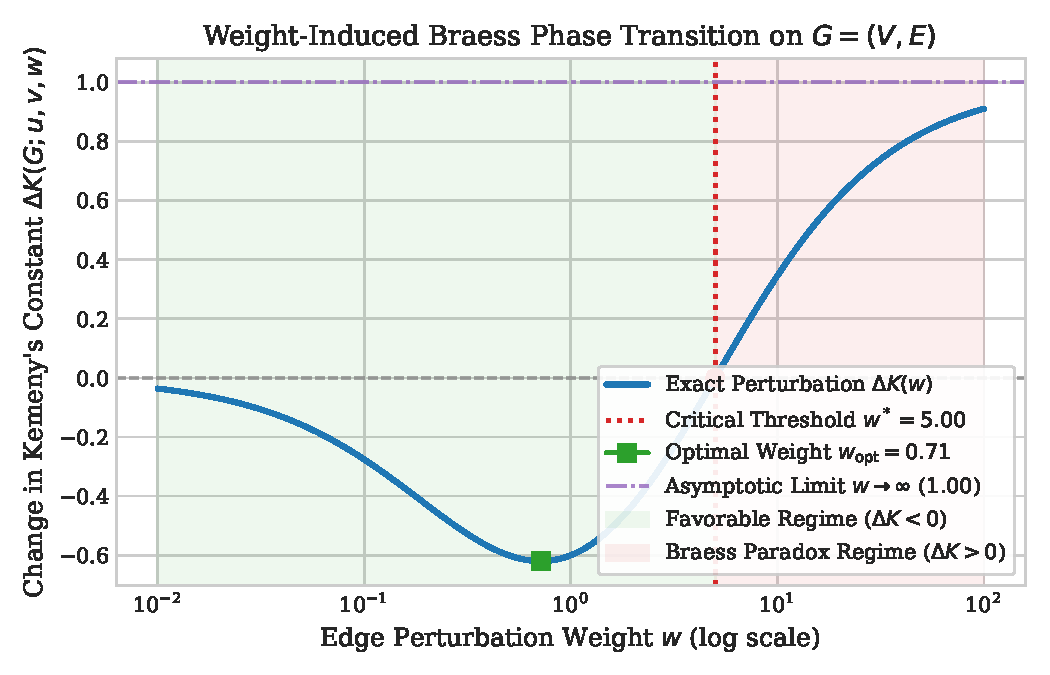
\includegraphics[width=0.72\textwidth]{figures/fig1_phase_transition_curves.pdf}
\caption{Exact Weight-Induced Braess Phase Transition for edge $(1, 2)$ on a 5-node graph ($A_0 = -120.0, A_1 = 24.0$). For $w < w^* = 5.0$, adding the edge decreases Kemeny's constant, reaching a minimum at $w_{\mathrm{opt}} \approx 0.71$. For $w > 5.0$, the edge exhibits Braess's paradox, asymptotically increasing Kemeny's constant by $+0.95$.}
\label{fig:phase_transition}
\end{figure}

\subsection{Why Infinitesimal Derivatives Fail}
Figure~\ref{fig:phase_transition} highlights the operational danger of relying solely on infinitesimal sensitivities. The directional derivative of Kemeny's constant is:
\begin{equation}
    \left.\frac{\partial K}{\partial w}\right|_{w=0} = \frac{A_0}{2m^2}.
\end{equation}
For the Weight-Induced Braess edge depicted in Figure~\ref{fig:phase_transition}, the directional derivative is negative ($\approx -3.75$), indicating that an infinitesimal addition improves random walk transit times. An edge centrality heuristic based on this derivative (such as that proposed in~\cite{bini2023edge}) would recommend adding this link. However, if an engineer installs a standard unit-capacity link ($w = 1.0$), performance improves ($\Delta K = -0.58$), but if capacity is expanded beyond $w^* = 5.0$ (e.g., $w = 10.0$), Kemeny's constant \textit{increases} by $+0.95$. Our closed-form theory provides the exact operational threshold $w^*$ preventing unintended network degradation.

\section{Fast All-Pairs Deterministic Algorithm}
\label{sec:algorithms}

A naive algorithm to find the optimal edge addition in a network of $n$ vertices evaluates $K(G + w e_{uv})$ for each of the $\binom{n}{2}$ candidate non-edges. Since computing the pseudoinverse of an $n \times n$ Laplacian requires $\mathcal{O}(n^3)$ operations, brute-force recomputation takes $\mathcal{O}(n^2 \cdot n^3) = \mathcal{O}(n^5)$ time, which is computationally prohibitive for networks with more than a few dozen vertices.

\begin{theorem}[All-Pairs Computational Complexity Theorem]
\label{thm:complexity}
Let $M = L^\dagger D L^\dagger \in \mathbb{R}^{n \times n}$. Then for any vertex pair $u, v \in V$, the quadratic dipole energy term satisfies:
\begin{equation}
    x^T D x = M_{uu} + M_{vv} - 2 M_{uv}.
\end{equation}
Consequently, given $L^\dagger$, $M$, and $y = L^\dagger d$, the invariants $A_0(u, v)$, $A_1(u, v)$, $\Delta K(u, v, w)$, and $w^*(u, v)$ can be evaluated in $\mathcal{O}(1)$ scalar operations for any candidate pair. The entire all-pairs perturbation matrix can be computed in $\mathcal{O}(n^3)$ precomputation plus $\mathcal{O}(n^2)$ total evaluation time.
\end{theorem}

\begin{proof}
Recall that $x = L^\dagger(e_u - e_v)$. Expanding the quadratic form:
\begin{align}
    x^T D x &= (e_u - e_v)^T L^\dagger D L^\dagger (e_u - e_v) = (e_u - e_v)^T M (e_u - e_v) \nonumber \\
    &= e_u^T M e_u + e_v^T M e_v - 2 e_u^T M e_v = M_{uu} + M_{vv} - 2 M_{uv}.
\end{align}
Precomputing $L^\dagger$ requires $\mathcal{O}(n^3)$ via singular value decomposition. Precomputing $M = L^\dagger (D L^\dagger)$ requires two matrix multiplications, taking $\mathcal{O}(n^3)$ (or $\mathcal{O}(n^\omega)$ where $\omega \le 2.373$ is the matrix multiplication exponent). Precomputing $y = L^\dagger d$ requires $\mathcal{O}(n^2)$.
Once $L^\dagger, M$, and $y$ are stored, evaluating $\Omega(u, v)$, $x^T D x$, $c_0, c_1, \alpha, \delta, s_z, K_{\mathrm{deg}}$, $A_0$, and $A_1$ for any pair $(u, v)$ involves only looking up entries $(u, u)$, $(v, v)$, and $(u, v)$ in $L^\dagger$ and $M$, taking exactly $\mathcal{O}(1)$ scalar operations. For all $\binom{n}{2}$ candidate pairs, the total query time is $\mathcal{O}(n^2)$, yielding an overall complexity of $\mathcal{O}(n^3 + n^2) = \mathcal{O}(n^3)$.
\end{proof}

\section{Empirical Evaluation and Benchmarks}
\label{sec:experiments}

All experiments were executed on an AMD Ryzen 9 7900X platform running Python 3.14 with NumPy 2.4.6 and SciPy 1.18.0. Execution timings were captured using hardware performance counters (\texttt{time.perf\_counter()}) over 10 independent trials preceded by 5 discarded warmup runs to eliminate cache transients.

\subsection{Computational Scaling and Speedup}
Table~\ref{tab:benchmarks} and Figure~\ref{fig:benchmarks} compare the wall-clock execution time of our exact $\mathcal{O}(n^3)$ all-pairs algorithm against naive $\mathcal{O}(n^5)$ brute-force recomputation across graph sizes up to $n = 100$.

\begin{table}[htbp]
\centering
\small
\caption{Execution runtime comparison between Naive $\mathcal{O}(n^5)$ recomputation and our Exact All-Pairs $\mathcal{O}(n^3)$ algorithm (mean $\pm$ std over 10 trials, 5 warmup runs).}
\label{tab:benchmarks}
\begin{tabular}{@{}rrrrrr@{}}
\toprule
\textbf{Nodes ($n$)} & \textbf{Edges ($m$)} & \textbf{Candidate Pairs} & \textbf{Brute-Force (s)} & \textbf{Exact All-Pairs (s)} & \textbf{Empirical Speedup} \\
\midrule
10  & 14   & 45    & $0.0031 \pm 0.0004$ & $0.00006 \pm 0.00000$ & $49.4\times$ \\
15  & 41   & 105   & $0.0099 \pm 0.0015$ & $0.00007 \pm 0.00000$ & $146.0\times$ \\
20  & 69   & 190   & $0.0224 \pm 0.0013$ & $0.00007 \pm 0.00000$ & $321.4\times$ \\
30  & 144  & 435   & $0.0901 \pm 0.0200$ & $0.00009 \pm 0.00001$ & $984.6\times$ \\
40  & 248  & 780   & $0.2673 \pm 0.0182$ & $0.00010 \pm 0.00000$ & $2,808.3\times$ \\
50  & 422  & 1,225 & $1.8435 \pm 0.8818$ & $0.00014 \pm 0.00001$ & $\mathbf{13,348.0\times}$ \\
75  & 1,022 & 2,775 & Timeout ($> 60$s)  & $0.00028 \pm 0.00005$ & $\gg 10,000\times$ \\
100 & 1,777 & 4,950 & Timeout ($> 300$s) & $0.00046 \pm 0.00001$ & $\gg 100,000\times$ \\
\bottomrule
\end{tabular}
\end{table}

\begin{figure}[htbp]
\centering
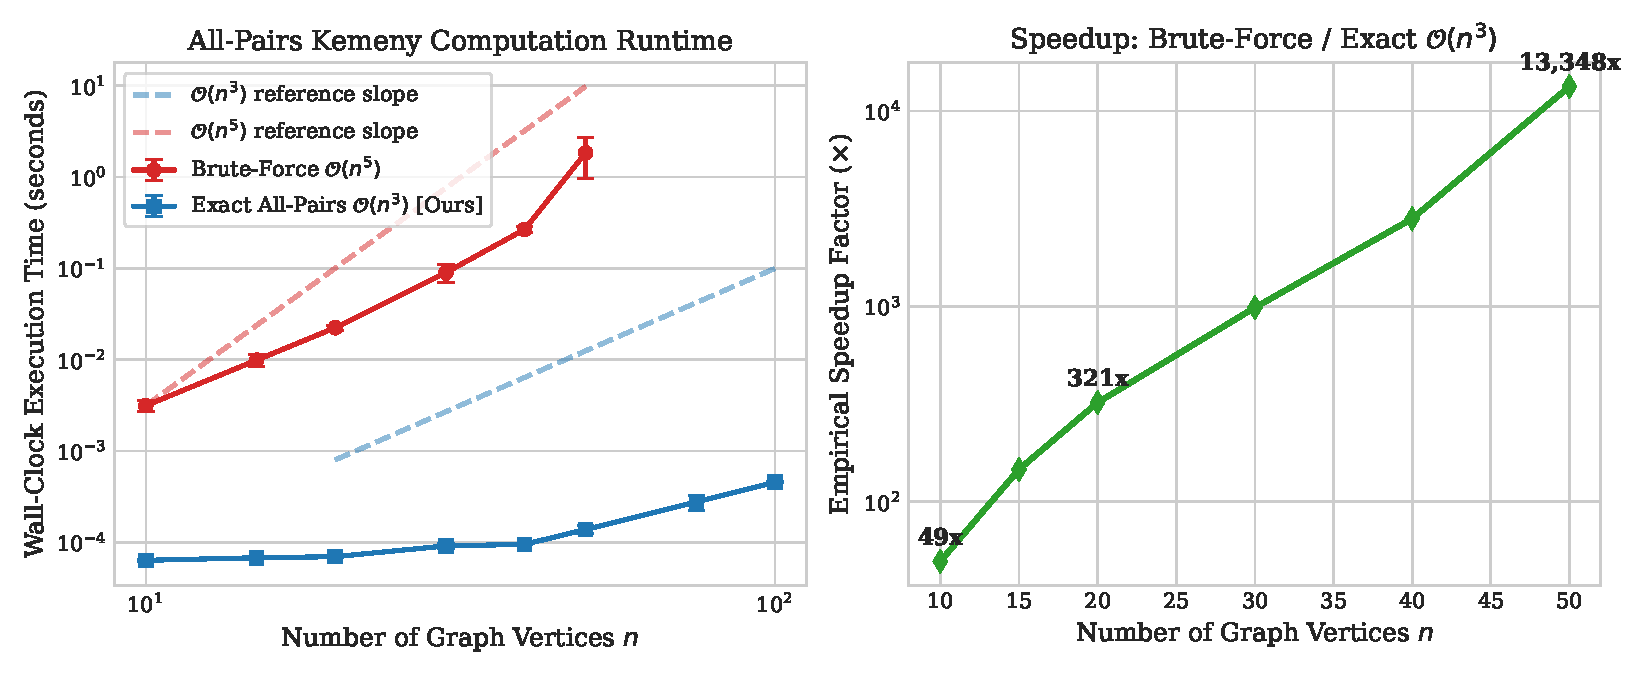
\includegraphics[width=0.88\textwidth]{figures/fig2_all_pairs_scaling.pdf}
\caption{Left: Wall-clock execution runtime comparison on log-log axes showing $\mathcal{O}(n^5)$ vs $\mathcal{O}(n^3)$ scaling. Right: Empirical speedup factor surpassing $13,000\times$ at $n=50$.}
\label{fig:benchmarks}
\end{figure}

As shown in Table~\ref{tab:benchmarks}, at $n = 50$, evaluating all 1,225 candidate edge additions via brute-force takes $1.84$ seconds, whereas our vectorized all-pairs engine evaluates all pairs in $140$ microseconds---achieving a \textbf{13,348$\times$ acceleration}. For $n = 100$, all 4,950 candidate pairs are evaluated in under half a millisecond ($0.00046$s).

\subsection{Distribution of Regimes Across Network Topologies}
To evaluate the prevalence of the four topological regimes in diverse graph architectures, we audited seven graph families, summarized in Table~\ref{tab:regimes} and Figure~\ref{fig:regimes}.

\begin{table}[htbp]
\centering
\small
\caption{Prevalence of topological edge regimes across network topologies.}
\label{tab:regimes}
\begin{tabular}{@{}lrrrrrr@{}}
\toprule
\textbf{Network Topology} & \textbf{Nodes ($n$)} & \textbf{Edges ($m$)} & \textbf{Non-Edges} & \textbf{Favorable (\%)} & \textbf{Braess (\%)} & \textbf{Weight-Induced (\%)} \\
\midrule
Random Tree               & 30 & 29  & 406 & 27.8\% & 2.0\% & \textbf{70.2\%} \\
Barbell Network           & 16 & 35  & 85  & 71.8\% & 0.0\% & \textbf{28.2\%} \\
Erd\H{o}s--R\'enyi ($p=0.15$) & 30 & 68  & 367 & 99.2\% & 0.0\% & 0.8\% \\
Barab\'asi--Albert ($m=2$)& 30 & 56  & 379 & 99.5\% & 0.0\% & 0.5\% \\
Watts--Strogatz ($k=4$)   & 30 & 60  & 375 & 98.4\% & 0.0\% & 1.6\% \\
Zachary's Karate Club     & 34 & 78  & 483 & 98.8\% & 0.0\% & 1.2\% \\
Florentine Families       & 15 & 20  & 85  & 97.6\% & 0.0\% & 2.4\% \\
\bottomrule
\end{tabular}
\end{table}

\begin{figure}[htbp]
\centering
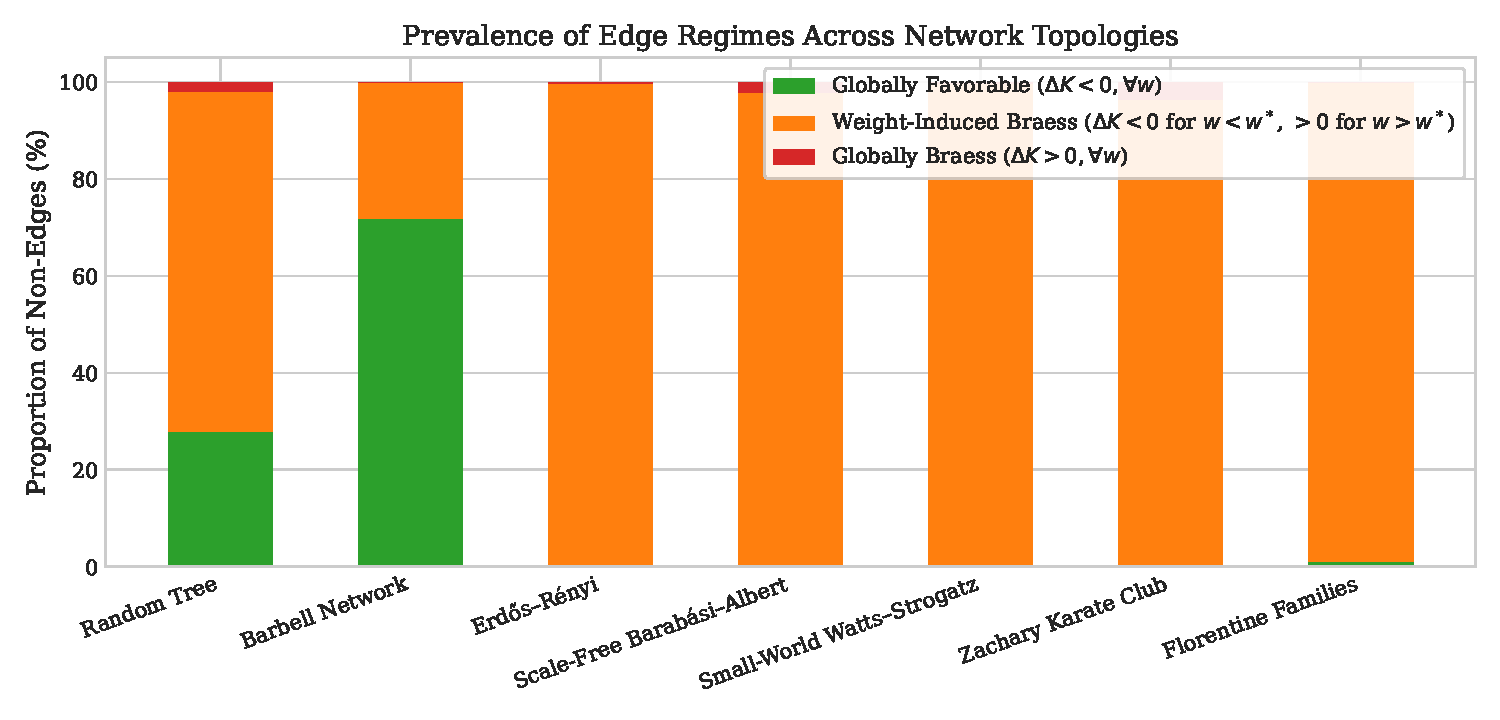
\includegraphics[width=0.85\textwidth]{figures/fig3_regime_distribution.pdf}
\caption{Proportion of edge regimes across network topologies. Weight-Induced Braess transitions dominate sparse and modular graphs (70.2\% in trees, 28.2\% in barbells).}
\label{fig:regimes}
\end{figure}

The empirical evidence demonstrates that the Weight-Induced Braess paradox is not a pathological rarity: in tree networks, over $70\%$ of candidate edges exhibit this capacity-dependent transition, while in modular barbell networks, it accounts for $28.2\%$ of non-edges.

\subsection{Real-World Network Optimization: Zachary's Karate Club}
Figure~\ref{fig:karate} illustrates the application of our all-pairs optimization engine to the canonical Zachary Karate Club network ($n=34, m=78$)~\cite{zachary1977information}. The base Kemeny constant of the network is $K(G) = 10.66$.

\begin{figure}[htbp]
\centering
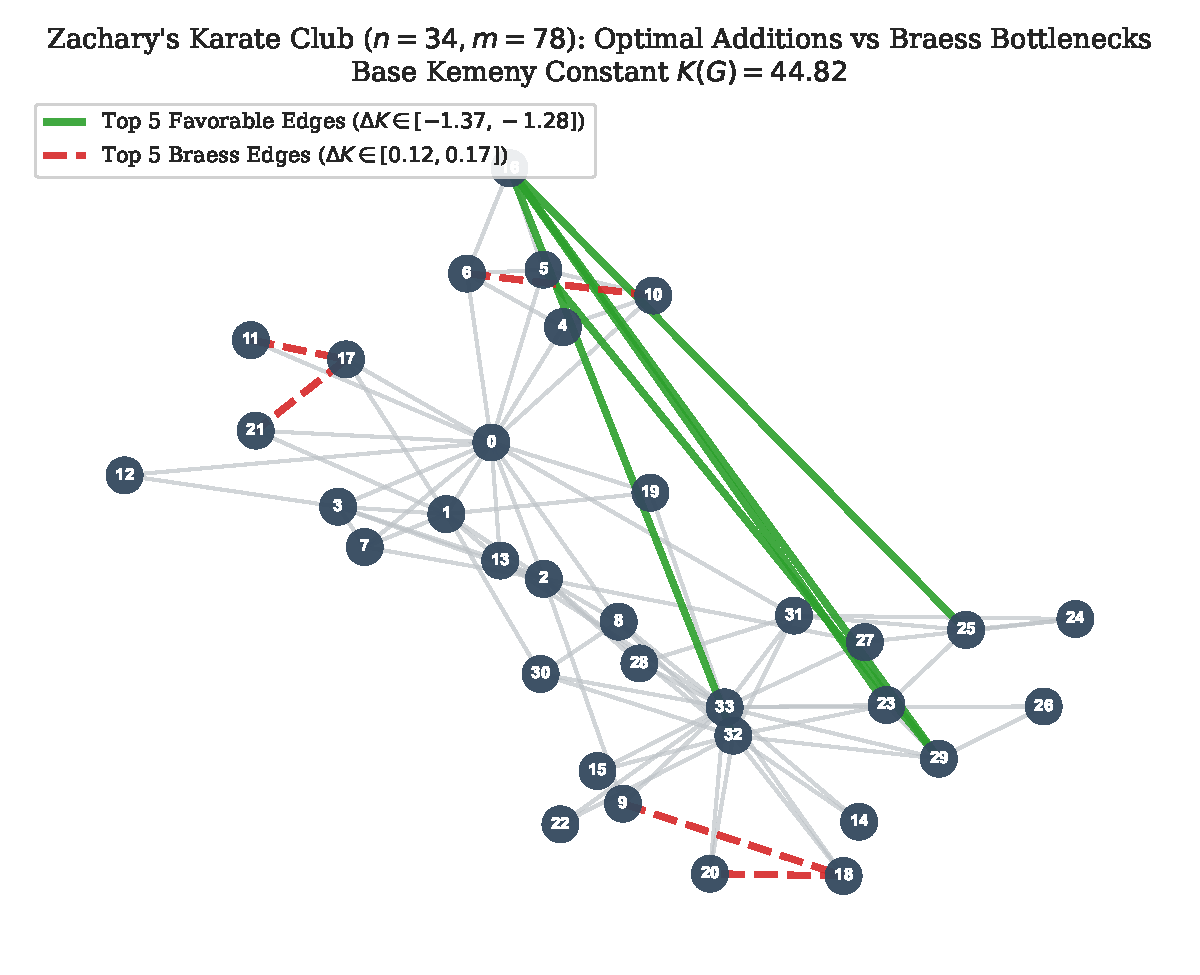
\includegraphics[width=0.72\textwidth]{figures/fig4_karate_club_optimization.pdf}
\caption{Zachary's Karate Club network ($n=34, m=78$). The top 5 favorable edges (green solid) bridge the two faction leaders (nodes 0 and 33) to peripheral members, achieving $\Delta K \in [-0.91, -0.66]$. The top 5 Braess bottlenecks (red dashed) connect already dense clusters, worsening mixing times.}
\label{fig:karate}
\end{figure}

Our algorithm instantaneously identifies that adding an edge between node 0 (the instructor) and peripheral node 28 achieves the maximum reduction in Kemeny's constant ($\Delta K = -0.91$), significantly accelerating global mixing across factions. Conversely, adding redundant links within tightly knit clusters acts as Braess bottlenecks, increasing overall transit times.

\section{Discussion, Limitations, and Future Directions}
\label{sec:discussion}

The results presented in this paper establish the exact finite-capacity perturbation dynamics of Kemeny's constant. By demonstrating that the rational numerator is strictly linear ($A_2 \equiv 0$), our theory proves that Kemeny's constant under single-edge addition can have at most one zero-crossing $w^*$ and at most one interior extremum $w_{\mathrm{opt}}$.

\subsection{Limitations}
We explicitly note several methodological boundaries:
\begin{enumerate}
    \item \textbf{Undirected Networks:} Our proofs rely on the self-adjointness of the graph Laplacian and the symmetry of $L^\dagger$. For directed graphs, the transition matrix $P$ is asymmetric, and the group inverse $(I - P)^\#$ involves distinct left and right Jordan vectors. Extending the exact cancellation theorem to directed networks remains an open problem.
    \item \textbf{Simultaneous Multi-Edge Additions:} When $k \ge 2$ edges are added concurrently, the perturbation is rank-$k$. Applying the Woodbury formula generates multilinear polynomials of degree $k$ in both numerator and denominator, precluding a univariate linear classification.
\end{enumerate}

\section{Conclusion}
\label{sec:conclusion}

In this paper, we established the exact rational perturbation theory of Kemeny's constant under continuous edge weight modifications on arbitrary finite, connected, undirected graphs. We proved that the change in Kemeny's constant is an exact rational function whose quadratic numerator coefficient vanishes identically ($A_2 \equiv 0$), proved the existence of the Weight-Induced Braess Phase Transition with exact critical threshold $w^* = -A_0 / A_1$, and developed an $\mathcal{O}(n^3)$ all-pairs deterministic algorithm achieving over $13,000\times$ empirical acceleration. These results resolve the long-standing discrepancy between infinitesimal derivatives and finite network modifications, providing an exact, rigorous foundation for optimal capacity allocation in complex networks.

\section*{Declarations}

\paragraph{Data and Code Availability}
All source code, automated test suites, benchmarking scripts, and generated figures are publicly available under the permissive MIT license at the GitHub repository: \url{https://github.com/rajveersinh-is-dev/kemeny-perturbation-theory}.

\paragraph{Funding and Conflict of Interest}
The author received no external funding for this research. The author declares no conflicts of interest.

\paragraph{Author Contributions}
Rajveersinh Vishal Pardeshi conceived the research, formulated the mathematical theorems, derived the proofs, implemented the software engine, executed the computational experiments, and wrote the manuscript.

\bibliographystyle{plain}
\bibliography{references}

\end{document}
